\RequirePackage{leftindex}
\documentclass[portrait]{tikzposter}

\usepackage{amsmath}
\usepackage{amsthm}
\usepackage{amssymb}
\usepackage{tikz}
\usepackage{multicol}
\usepackage{cancel}


\DeclareMathOperator{\st}{st}
\DeclareMathOperator{\diff}{d}

\newcommand{\ls}{\leftindex^*}

\newcommand{\NN}{\mathbb{N}}
\newcommand{\ZZ}{\mathbb{Z}}
\newcommand{\QQ}{\mathbb{Q}}
\newcommand{\RR}{\mathbb{R}}
\newcommand{\HR}{\ls\RR}

\newcommand{\itemrule}{\vspace{0.5cm}\hrule\vspace{0.3cm}}

\theoremstyle{definition}
\newtheorem*{definition}{Definition}
\newtheorem*{example}{Example}

\theoremstyle{plain}
\newtheorem*{theorem}{Theorem}

\theoremstyle{remark}
\newtheorem*{remark}{Remark}

\title{\parbox{\linewidth}{\centering Calculus without Limits \\ \huge The Formation of Nonstandard Analysis}}
\author{Eason Shao}
\institute{St Paul's School}
\date{\today}

\usetheme{Board}

\begin{document}

\maketitle

\begin{columns}
    \column{0.6}
    \block{History of Infinitesimals}{

        \begin{itemize}
            \item c. 250 B.C., Archimedes: Infinities and infinitesimals.
                  \begin{theorem}[Archimedes Property of the Real Numbers \(\RR\)]
                      For any two real numbers \(x, y \in \RR\), \(x, y > 0\), there exists a natural number \(n \in \NN\), such that \(nx > y\).

                      In other words, for any two positive real numbers, some multiple of one must be greater than the other.
                  \end{theorem}

                  Essentially, no infinities or infinitesimals exist in the real number set \(\RR\).

                  In other words, \(y\) is an infinity if any multiple of a real number \(x \in \RR\) is less than \(y\). Infinitesimals can be defined similarly.

                  \itemrule

            \item c. 1660, Newton, Leibnitz: Formulation of Non-rigorous Calculus with Infinitesimals.

                  \begin{example}
                      They argue that the derivative of \(f(x) = x^2\) is \(f'(x) = 2x\), since
                      \[
                          \frac{f(x + o) - f(x)}{o} = \frac{(x + o)^2 - x^2}{o} = \frac{2 x \cancel{o} + \cancel{o}^2}{\cancel{o}} = 2x + o = 2x.
                      \]

                      We can cancel out the \(o\) on the top and bottom since it is non-zero.

                      But since \(o\) is infinitesimal, it is \(0\), which gives \(2x\).
                  \end{example}

                  It is inconsistent (and caused the second mathematical crisis) since sometimes \(o \neq 0\) and sometimes \(o = 0\).

                  \itemrule

            \item c. 1820, Cauchy, Weierstrass: Formal definition of a limit (\(\epsilon-\delta\)).

                  \begin{definition}[The \(\epsilon-\delta\) definition of a limit]
                      The limit of \(f(x)\) as \(x\) tends to \(c\) is A, or \( \lim_{x \rightarrow c} f(x) = A,\) if and only if, for all \(\epsilon > 0\), there exists a \(\delta > 0\), such that for all \(0 < |x - c| < \delta\), we have \(|f(x) - A| < \epsilon\).
                  \end{definition}

                  It is very formal and rigorous but less intuitive to understand.

                  \itemrule

            \item 1934, Skolem: First development of non-standard analysis.
            \item 1948, E. Hewitt and 1955, J. Los: Formation of non-standard analysis.
            \item 1961, A. Robinson: A mathematical (rigorous) interpretation of continuity and infinitesimals (hyperreals) based on work by Hewitt and Los.
        \end{itemize}
    }

    \block{Visuallization of Hyperreals}{
        \begin{center}
            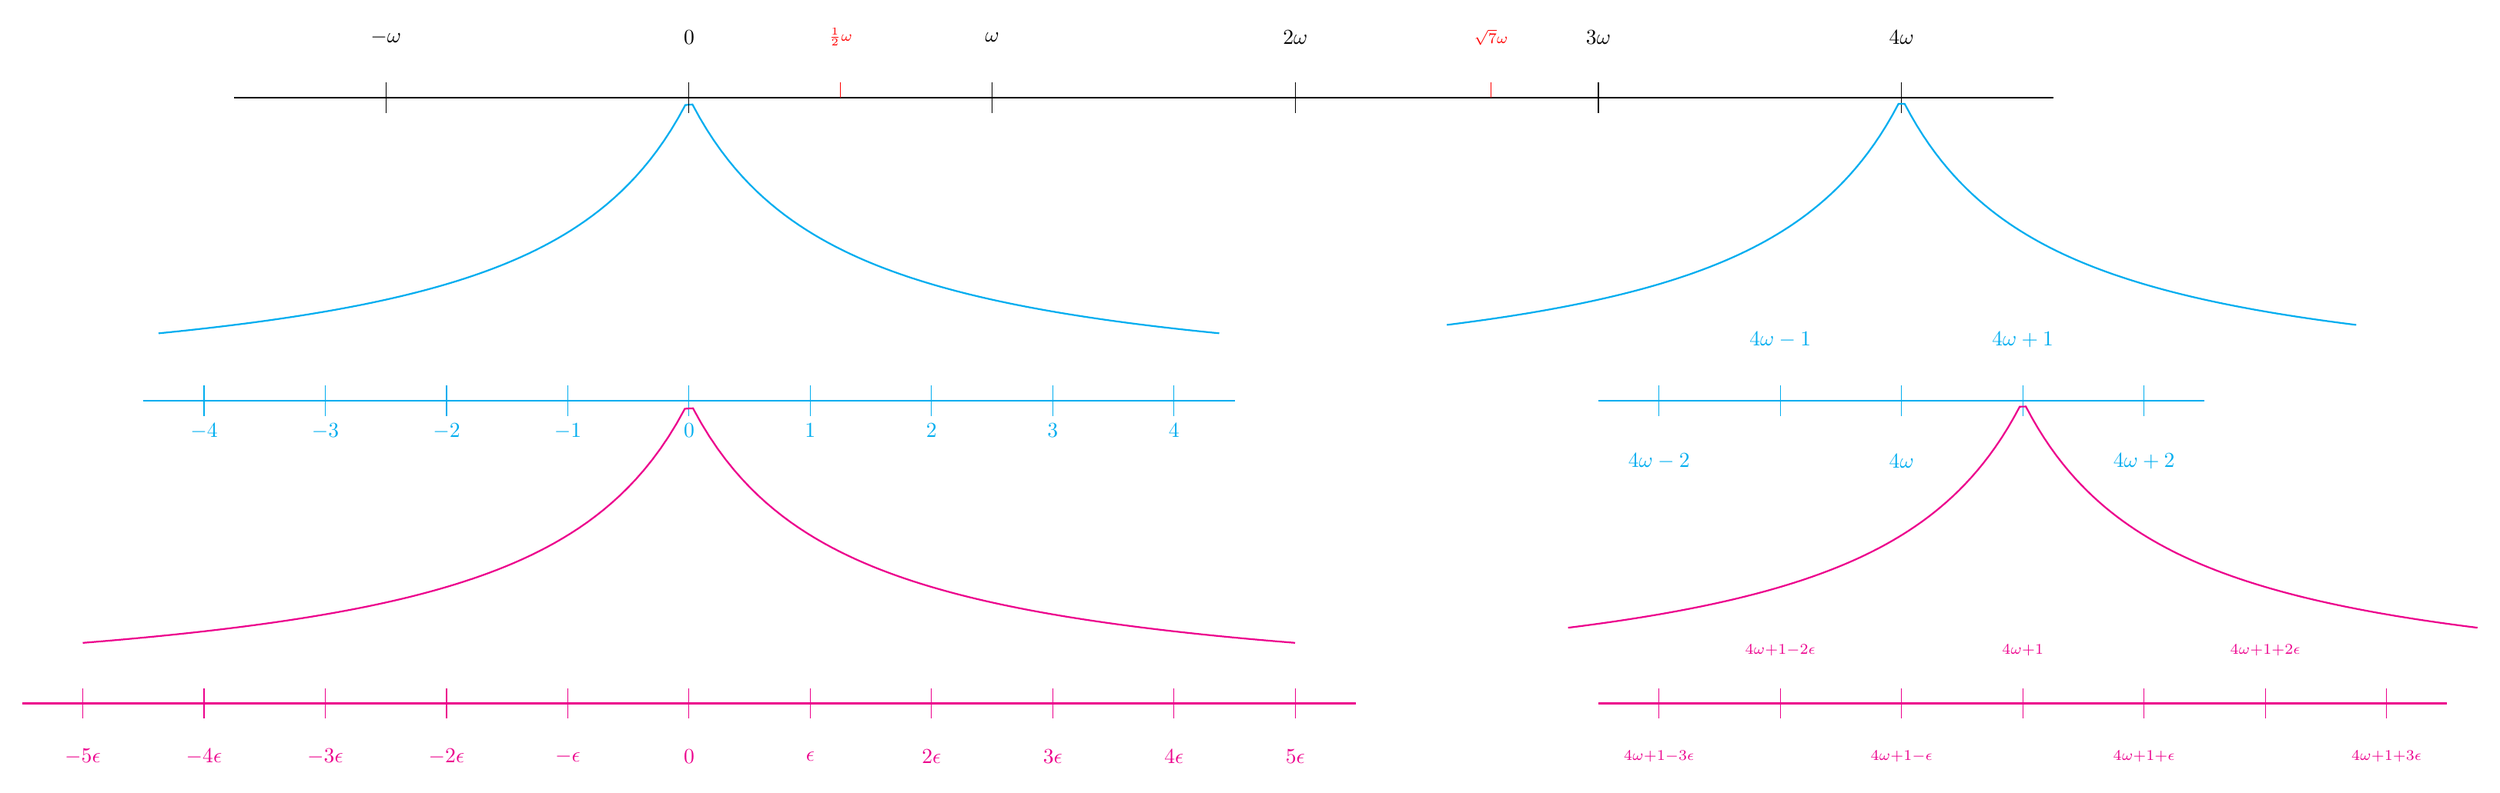
\begin{tikzpicture}[scale=2.5]
                \draw [color = cyan, thick] (-3.6, 3) -- (3.6, 3);
                \foreach \x in {-4, -3, -2, -1, 0, 1, 2, 3, 4}
                \draw [color = cyan] (\x * 0.8, 3.1) -- (\x * 0.8, 2.9) node[below] {\(\x\)};

                \draw[thick, magenta] plot[domain = -4:4, samples = 150] (\x,{2 / (abs(\x) + 1) + 1});

                \draw [color = magenta, thick] (-4.4, 1) -- (4.4, 1);
                \foreach \x in {-5, -4, -3, -2, -1, 0, 1, 2, 3, 4, 5}
                \draw [color = magenta] (\x * 0.8, 1.1) -- (\x * 0.8, 0.9);

                \foreach \x in {-5, -4, -3, -2, 2, 3, 4, 5}
                \node [color = magenta] at (\x * 0.8, 0.65) {\(\x\epsilon\)};

                \node [color = magenta] at  (-1 * 0.8, 0.65) {\(-\epsilon\)};
                \node [color = magenta] at (0 * 0.8, 0.65) {\(0\)};
                \node [color = magenta] at (1 * 0.8, 0.65) {\(\epsilon\)};

                \draw[thick, cyan] plot[domain = -3.5:3.5, samples = 150] (\x, {2 / (abs(\x) + 1) + 3});

                \draw [thick] (-3, 5) -- (9, 5);
                \foreach \x in {-1, 0, 1, 2, 3, 4}
                \draw (\x * 2, 5.1) -- (\x * 2, 4.9);

                \foreach \x in {2, 3, 4}
                \node at (\x * 2, 5.4) {\(\x\omega\)};

                \node at (-2, 5.4) {\(-\omega\)};
                \node at (0, 5.4) {\(0\)};
                \node at (2, 5.4) {\(\omega\)};

                \draw [color = red] (1, 5.1) -- (1, 5);
                \node [color = red] at (1, 5.4) {\(\scriptstyle\frac{1}{2}\omega\)};

                \draw [color = red] (5.2915026221, 5.1) -- (5.2915026221, 5);
                \node [color = red] at (5.2915026221, 5.4) {\(\scriptstyle \sqrt{7}\omega\)};

                \draw[thick, cyan] plot[domain = -3:3, samples = 150] (\x + 8, {2 / (abs(\x) + 1) + 3});

                \draw [color = cyan, thick] (6, 3) -- (10, 3);
                \foreach \x in {-2, -1, 0, 1, 2}
                \draw [color = cyan] (\x * 0.8 + 8, 3.1) -- (\x * 0.8 + 8, 2.9);

                \node [color = cyan] at (-2 * 0.8 + 8, 2.6) {\(4\omega - 2\)};
                \node [color = cyan] at (-1 * 0.8 + 8, 3.4) {\(4\omega - 1\)};
                \node [color = cyan] at (0 * 0.8 + 8, 2.6) {\(4\omega\)};
                \node [color = cyan] at (1 * 0.8 + 8, 3.4) {\(4\omega + 1\)};
                \node [color = cyan] at (2 * 0.8 + 8, 2.6) {\(4\omega + 2\)};

                \draw[thick, magenta] plot[domain = -3:3, samples = 150] (\x + 8.8,{2 / (abs(\x) + 1) + 1});

                \draw [color = magenta, thick] (6, 1) -- (11.6, 1);
                \foreach \x in {-3, -2, -1, 0, 1, 2, 3}
                \draw [color = magenta] (\x * 0.8 + 8 + 0.8, 1.1) -- (\x * 0.8 + 8 + 0.8, 0.9);

                \node [color = magenta] at (-3 * 0.8 + 8 + 0.8, 0.65) {\(\scriptstyle 4\omega + 1 - 3\epsilon\)};
                \node [color = magenta] at (-2 * 0.8 + 8 + 0.8, 1.35) {\(\scriptstyle 4\omega + 1 - 2\epsilon\)};
                \node [color = magenta] at (-1 * 0.8 + 8 + 0.8, 0.65) {\(\scriptstyle 4\omega + 1 - \epsilon\)};
                \node [color = magenta] at (0 * 0.8 + 8 + 0.8, 1.35) {\(\scriptstyle 4\omega + 1\)};
                \node [color = magenta] at (1 * 0.8 + 8 + 0.8, 0.65) {\(\scriptstyle 4\omega + 1 + \epsilon\)};
                \node [color = magenta] at (2 * 0.8 + 8 + 0.8, 1.35) {\(\scriptstyle 4\omega + 1 + 2\epsilon\)};
                \node [color = magenta] at (3 * 0.8 + 8 + 0.8, 0.65) {\(\scriptstyle 4\omega + 1 + 3\epsilon\)};
            \end{tikzpicture}

        \end{center}
    }

    \column{0.4}
    \block{Transfer Principle}{
        To develop a number system that includes infinities and infinitesimals and to make it useful (and intuitive) at the same time, we really would like as many properties to preserve from \(\mathbb{R}\) to this number set, \textbf{hyperreal numbers} \(\HR\) as possible.

        \begin{theorem}[Transfer Principle from \(\RR\) to \(\HR\)]
            Any statement of the form "for any number \(x\) ..." that is true for the reals \(x \in \RR\) is also true for the hyperreals \(x \in \HR\).
        \end{theorem}

        \vspace{2cm}

    }

    \note[
        targetoffsetx=-8cm,
        targetoffsety=-5cm,
        width=0.35\linewidth
    ]
    {
        Statements on sets and functions might not hold since they might depend on specific properties of real numbers.
    }

    \block{Hyperreal Numbers}{
        Luckily, such formation does indeed exist!

        \begin{definition}[Hyperreal Numbers]
            The \textbf{hyperreal numbers} \(\HR\) are defined to be the real numbers \(\RR\), together with:
            \begin{itemize}
                \item \textbf{Infinitesimals} which have (absolute value) smaller than any real number.
                \item \textbf{Infinities} which have (absolute value) larger than any real number.
            \end{itemize}
            We define \(\omega\) as an infinity, and \(\epsilon\) as an infinitesimal:
            \[\epsilon = \frac{1}{\omega}, \epsilon \omega = 1.\]
        \end{definition}

        \begin{example}
            \begin{enumerate}
                \item For any real number \(x, y \in \RR\), we have \(x + y = y + x\). (Commutativitiy of Addition over \(\RR\)).

                      This also holds for hyperreal numbers \(x, y \in \HR\). We will have \(\omega + 1 = 1 + \omega\), and things like \(\epsilon^2 + \omega  = \omega + \epsilon^2\).
                \item For any real number \(x, y, z \in \RR\), \(y, z \neq 0\), we have \(\frac{x}{y} = \frac{xz}{yz}\).

                      This also holds for hyperreal numbers \(x, y, z \in \HR\) satisfying \(y, z \neq 0\). We will have, for example,
                      \[
                          \frac{1}{1 + \epsilon} = \frac{1 - \epsilon}{1 - \epsilon^2}.
                      \]
            \end{enumerate}
        \end{example}
    }

    \block{Standard Part}{
        \begin{definition}[Standard Part]
            If some hyperreal number \(x \in \HR\) and is finite, then we define the function \(\st\), as
            \[
                \st (x) = \text{the closest real number to \(x\)}.
            \]
        \end{definition}

        \begin{example}
            \(\st (2 + \epsilon) = 2\), \(\st (3 - \epsilon + \epsilon^4) = 3\).
        \end{example}

    }

\end{columns}

\begin{columns}

    \column{0.5}

    \block{Derivative}{
        For a function \(f\), we defined its derivative using First Principles:
        \begin{definition}[First Principles]
            \[
                f'(x) = \lim_{h \rightarrow 0} \frac{f(x+h) - f(x)}{h}.
            \]
        \end{definition}

        Here, \(h\) is just an infinitesimal, and so we can define the derivative using hyperreals:
        \begin{definition}[Derivative from Hyperreals]
            \[
                f'(x) = \st\left(\frac{f(x + \epsilon) - f(x)}{\epsilon}\right).
            \]
        \end{definition}


        \begin{example}
            If we set \(f(x) = x^n\), we try and find \(f'\) using this.
            \begin{align*}
                f'(x) & = \st\left(\frac{(x+\epsilon)^n - x^n}{\epsilon}\right)                                                                                                \\
                      & = \st\left(\frac{\left(x^n + n \epsilon x^{n-1} + \frac{n(n-1)}{2}\epsilon^2 x^{n - 2} + \ldots\right) - x^n}{\epsilon}\right)                         \\
                      & = \st\left(\frac{n \epsilon x^{n-1} + \frac{n(n-1)}{2}\epsilon^2 x^{n - 2} + \ldots}{\epsilon}\right) = \st \left(n x^{n-1} + \square \epsilon\right),
            \end{align*}

            where \(\square\) is something that is not infinity.

            So \(\square \epsilon\) must be an infinitesimal, and therefore \(f'(x) = n x^{n-1}\).
        \end{example}
    }

    \column{0.5}

    \block{Limits}{
        \begin{definition}[Limits]
            We define
            \[
                \lim_{x \rightarrow +\infty} f(x) = \st(f(\omega)), \lim_{x \rightarrow -\infty} f(x) = \st(f(-\omega)).
            \]
            and
            \[
                \lim_{x \rightarrow a^{+}} f(x) = \st(f(a + \epsilon)), \lim_{x \rightarrow a^{-}} f(x) = \st(f(a - \epsilon)).
            \]
        \end{definition}

        It is soon apparent that this and the First Principle give the exact definition of the derivative. If we recall the definition of \(e\):
        \begin{definition}[\(e\)]
            \[
                e = \lim_{x \rightarrow \infty} \left(1 + \frac{1}{x}\right)^x = \st \left(\left(1 + \frac{1}{\omega}\right)^\omega\right)  = \st \left(\left(1 + \epsilon\right)^\omega\right),
            \]
        \end{definition}
        we try to find the derivative of \(g(x) = e^x\).

        \begin{example}
            \begin{align*}
                g'(x) & = \st \left(\frac{e^{x + \epsilon} - e^x}{\epsilon}\right)
                = e^x \st \left(\frac{e^\epsilon - 1}{\epsilon}\right)                                          \\
                      & = e^x \st \left(\frac{\left(1 + \epsilon \right)^{\omega\epsilon} - 1}{\epsilon}\right) \\
                      & = e^x \st \left(\frac{1 + \epsilon - 1}{\epsilon}\right)                                \\
                      & = e^x \st (1) = e^x.
            \end{align*}
        \end{example}
    }

\end{columns}

\block{Limitation}{
    \begin{multicols}{2}
        There is a famous function called the \textbf{Dirichlet Function}, which is not continuous at any point.

        \begin{definition}[Dirichlet Fucntion]
            The \textbf{Dirichlet Function} \(D: \RR \rightarrow \{0, 1\}\) is defined as
            \[
                D(x) = \begin{cases}
                    1, & x \in \QQ,               \\
                    0, & x \in \RR \setminus \QQ.
                \end{cases}
            \]
        \end{definition}

        It is difficult to formalize this limit using hyperreals intuitively since we did not classify hyperreals as rational and irrational - things like \(D(\epsilon)\) are not defined.

        If we use the standard part of \(x\) to define \(D(x)\), i.e., \(\ls D (x) = D(\st(x)),\)
        then this will give ridiculous results such as \(D\) is continuous at every point, which does not make sense.

        \vspace{2cm}
    \end{multicols}
}

\note[
    targetoffsetx=11cm,
    targetoffsety=-3cm,
    width=0.5\linewidth
]
{There is a way in which hyperreal numbers can be formalized, using hypernatural and hyperrational numbers. However, at this point, we might as well just go back to the \(\epsilon-\delta\) definition of the limit.}

% \block{References}{\printbibliography}

\end{document}